
\chapter{Introduction}
%=====================

Intel owns an Internet-scale distributed compute farm that is used for
running its massive chip-simulation workloads
\citet[p.\ 78]{bentley01,evans03:book}.
The farm is composed of tens of thousands of servers that are located
in multiple data centers that are geographically spread around the
globe.
It is capable of running hundreds of thousands of simulation jobs and
tests simultaneously, and handles a rate of thousands of newly
incoming jobs every second.

This huge compute capacity is managed by an in-house developed
highly-scalable two-tier resource management and scheduling system
called \nb.
At the lower level \nb\ groups the servers into autonomous clusters
that are referred to in \nb\ terminology as Physical Pools.
Each such pool contains up to thousands of servers and is managed by a
single \nb\ entity that is called the Physical Pool Manager or PPM.
The role of the PPM is to accept jobs from the upper level, and to
schedule them on underlying servers efficiently and with minimal
waste.

At the upper level \nb\ deploys a second set of pools that are called
Virtual Pools.
Just like in the lower level, each virtual pool is managed by a single
\nb\ component that is called the Virtual Pool Manager or VPM.
The role of the VPMs is to cooperatively accept jobs from the users
and distribute them to the different PPMs in order to spread the load
across the farm.
Together, these two layers, VPMs at the top and PPMs at the
bottom, strive to utilize every compute resource across the farm.
This paper focuses on the work done at the PPM level.

A basic requirement in \nb\ is the enforcement of fair-share
scheduling among the various projects and business units within Intel
that share the farm.
Fair-share begins at the planning phase where different projects
purchase different amounts of servers to be used for their jobs.
These purchases eventually reflect their share of the combined
resources.
Once the shares are calculated, they are propagated to the PPMs where
they are physically enforced. (The calculation and propagation
mechanisms are beyond the scope of this paper.)

To enforce fair-share the PPM constantly monitors which jobs from
which projects are currently running and the amount of resources they
use.
The PPM then selects from its wait queue the first job from the most
eligible project (the project whose ratio of currently used resources
to its share of the resources is the smallest) and tries to match a
machine to that job.
If the matching succeeds, the job is scheduled for execution on that
machine.
Otherwise, a reservation is made for the job, and the process is
repeated while making sure not to violate previously made
reservations.
Such reservations enable jobs from projects that are lagging behind to
obtain the required resources as soon as possible.

Matching machines to jobs is done using any of a set of heuristics.
For example, one may sort the list of candidate machines according to
some pre-defined criteria --- e.g.\ increasing number of free cores or
decreasing amount of free memory --- and then traverse the sorted list
and select the first machine on which the job fits.
This leads to variants of \bef\ and \wof\ schemes.
Good sorting criteria reduce fragmentation thus allowing more jobs to be
executed, and are critical for the overall utilization of the pool.
Alternatively one may opt to reduce overhead and use a
\fif\ heuristic.

The sorting criteria are programmable configuration parameters in \nb.
This allows one to implement various matching heuristics and apply
them on different resources to best suit the workload characteristics
and needs.
\nb\ also allows individual jobs to specify different heuristics,
while the pool administrator can set a default policy to be used for
all jobs.

In this paper we argue that no heuristic applied to a
single resource in isolation can yield optimal performance under all
scenarios and cases.
To demonstrate our point we use both simple test cases and workload
traces that were collected at four large Intel sites.
Using the traces, we simulate the PPM behavior when applying the
different heuristics to schedule the jobs.
We show that depending on the workload different heuristics may be
capable of scheduling a higher number of jobs.

In an attempt to overcome the problem we develop ``\mif'' --- a
combined heuristic that tries to balance the use of cores and memory.
Intuitively this should reduce fragmentation at the pool.
However, while generally better than the previous heuristics,
\mif\ too fails to yield optimal assignments in some cases.

As an alternative, we propose a meta-heuristic we call ``\maj''.
\maj\ is not tailored towards specific workloads or configurations.
Instead, it uses the aforementioned heuristics as sub-routines and
chooses, in every scheduling cycle, the one that yields the highest
number of matched jobs.
This overcomes corner cases that hinder specific heuristics from being
optimal in all cases, and conforms well to the \nb\ philosophy of
maximizing resource utilization in every step.
We demonstrate, through simulation, that \maj\ yields lower wait times
by up to 22\% for all jobs in average under high loads.
%Interestingly, we also find that \mif\ produces scheduling decisions
%that are very close to those of \maj.

The rest of this paper is organized as follows.
Section \ref{sec:matching} provides more details on the problem of
matching machines to jobs, and explores the performance of commonly
used heuristics.
Section \ref{sec:mixed-fit} then describes the \mif\ heuristic,
followed by the \maj\ meta-heuristic in Section \ref{sec:max-jobs},
and simulation results in Section \ref{sec:sim_results}.
Section \ref{sec:related} briefly presents related work, and Section
\ref{sec:conclusions} concludes the paper.



\chapter{Matching Machines to Jobs}
%==================================
\label{sec:matching}

As described above, matching machines to jobs at the PPM is done by
choosing the most eligible job from the wait queue, sorting the list
of candidate machines according to some pre-defined criterion,
traversing the sorted list, and selecting the first machine on which
the job fits\footnote{This is done for practical reasons since trying
  all combinations is time consuming.}.
This is repeated again and again until either the wait queue or the
list of machines are exhausted.
At this point the PPM launches the chosen job(s) on the selected
machine(s) and waits for the next scheduling cycle.

A job may be multithreaded, but we assume that each job can fit on a
single (multicore) machine.
In principle \nb\ also supports parallel jobs (called ``MPI jobs'')
that span multiple machines, but in practice their numbers at the
present time are small.
The only added difficulty in supporting such jobs is the need to
allocate multiple machines at once instead of one at a time.

%Selecting the optimal match of jobs to machines is difficult problem that
%may be time consuming. Since scheduling cycles are short, and  \nb\
%strive to reduce the overhead of that calculation, a heuristic is employed
%to sort the machines. 
There are many criteria by which the machines can be sorted.
In this paper we focus on the number of free cores and amount of free
memory, as this suits well the workload in Intel which is
characterized by compute-intensive memory-demanding jobs.
Though I/O is definitely a factor, and some jobs do perform large file
operations, there are some in-house solutions that are beyond the
scope of this paper that greatly reduce the I/O burden on the
machines.

\begin{figure}[p]\centering
%	\includegraphics[width=.9\textwidth]{figures/cores_multiplot.eps}
	\includegraphics{figures/cores_multiplot.eps}
\caption{Jobs' cores requirements: the vast majority of the jobs are
  serial and require a single CPU core in order to execute.}
\label{fig:cores_usage_multiplot}
%\end{figure}
%\begin{figure}\centering
%	\includegraphics[width=1.0\textwidth]{figures/memory_multiplot.eps}
	\includegraphics{figures/memory_multiplot.eps}
\caption{Jobs' memory requirements: demands are mostly 8 GB and below,
  but there are jobs that require 16 GB, 32 GB or even more memory in
  order to execute.}
\label{fig:memory_usage_multiplot}
\end{figure}

%At Intel, job is a process that is submitted with a definition of
%processors and memory requirements for its execution. Job can be parallel and
%require one or few cores, and a specific amount of memory in GB. 
Figures \ref{fig:cores_usage_multiplot} and \ref{fig:memory_usage_multiplot}
show the distribution of the jobs' cores and memory requirements in four large pools at different locations across the Intel farm%
\footnote{The requirements are specified as part of the job profile at submit time.}.
The data comes from traces \cite{parallel13} that were collected at the PPM
level during a one-month period, and which contain up to 13 million jobs each.
As can be seen in the figures, the vast majority of the jobs are
serial (single-thread jobs, requiring a single CPU core in order to execute).
Memory requirements are mostly 8 GB and below, but there are jobs that
require 16 GB, 32 GB, or even more memory (not shown) in order to
execute.
These observations are consistent across the pools.

%Figure \ref{fig:cores_mem_dist} shows the distribution of the jobs' cores and memory requirements in one of Intel's largest pools. The data comes from a trace that was collected during a one-month period and which contains more than 13 million jobs. As can be seen in Figure \ref{fig:cores_dist}, the vast majority of the jobs are serial and require a single CPU core in order to execute. Memory demands are mostly 8GB and below, but there are jobs that require 16GB, 32GB, or even more memory (not shown) in order to execute.

%\begin{figure}\centering
%\subfigure[\label{fig:cores_dist}Jobs' cores requirements]{
%	\includegraphics[width=0.45\textwidth]{figures/cores.eps}}
%\subfigure[\label{fig:mem_dist}Jobs' memory requirements]{
%	\includegraphics[width=0.45\textwidth]{figures/memory.eps}}
%\caption{Jobs' cores and memory requirements: (a) the vast majority of the jobs are serial and require a single CPU core in order to execute. (b) Memory demands are mostly 8GB and below, but there are jobs that require 16GB, 32GB or even more memory in order to execute.}
%\label{fig:cores_mem_dist}
%\end{figure}


The two ways to sort the machines by available cores or memory are in
increasing or decreasing order.
Sorting them by \textit{increasing} amount of free cores or memory and
selecting the first machine on which the job fits effectively
implements the \bef\ heuristic.
\bef\ is known to result in a better packing of jobs, while
maintaining unbalanced cores (or memory) usage across the machines in
anticipation for future jobs with high resource requirements.
Sorting the machines by \textit{decreasing} amount of free cores or
memory implements the \wof\ heuristic.
\wof's advantage is in keeping resource usage balanced across
machines, which is particularly useful for mostly-homogeneous
workloads.
For completeness we also mention \fif.
\fif's advantage is in its simplicity, as it does not require the
sorting of the machines.
Our tests, however, revealed that it performs poorly in our
environment, so we do not refer to it further in this paper.

We argue that no single heuristic, when applied to a single resource in
isolation, can yield optimal performance under all workload
scenarios.
To demonstrate our point we begin by providing simple synthetic examples
showing how different heuristics match different number of jobs under
different workload conditions.
We then put theory to the test by running simulations on the
aforementioned traces, demonstrating the effectiveness of the different heuristics 
under different workloads.


\section{Synthetic Examples of Heuristics Failures}
%-----------------------------------------------------

In our examples we consider two machines, A and B, each having four
cores and 32 GB of memory.
Assume that 8 jobs are queued at the PPM in the following priority order: two jobs
of one core and 16 GB of memory, and then 6 jobs of one core and 4 GB of
memory.
As can be seen in Figure \ref{fig:wf_better_A}, \bef\ matches the first
two jobs with machine A, totally exhausting its memory, and the next
four jobs with machine B, thereby exhausting its cores.
The end result is two unutilized cores on machine A, half the memory
unutilized on machine B, and two jobs that remain pending at the PPM.
\wof\ on the other hand matches the first two jobs on different
machines, which leaves enough free space (cores and memory) for all the
remaining 6 jobs to be matched.
This is illustrated in Figure \ref{fig:wf_better_B}.

\begin{figure}\centering
\subfigure[\label{fig:wf_better_A}\bef]{
	\includegraphics[width=0.45\textwidth]{figures/fig1a.eps}}
~~~~
\subfigure[\label{fig:wf_better_B}\wof]{
	\includegraphics[width=0.45\textwidth]{figures/fig1b.eps}}
\caption{Scenario for which \wof\ (right) is better than \bef\ (left).
  Memory is depicted in 4 GB blocks.
  Shading indicates mapping of a job to a certain core and certain
  blocks of memory.
  Note that both cores and memory are mapped exclusively to distinct
  jobs.}
\label{fig:wf_better}
\end{figure}

Another example is illustrated in Figure \ref{fig:bf_better}.
The priority order here is 3 jobs of one core and 8 GB, followed by
one job of one core and 32 GB of memory.
As can be seen, \wof\ spreads the first three jobs on different
machines, which doesn't leaves enough memory for the 32 GB job to be
matched.
\bef\ on the other hand matches the first three jobs on machines A, 
which allows the 32 GB to be matched with machine B.

\begin{figure}\centering
\subfigure[\label{fig:bf_better_A}\bef]{
	\includegraphics[width=0.45\textwidth]{figures/fig2b.eps}}
~~~~
\subfigure[\label{fig:bf_better_B}\wof]{
	\includegraphics[width=0.45\textwidth]{figures/fig2a.eps}}
\caption{Scenario for which \bef\ (left) is better than \wof\ (right). }
\label{fig:bf_better}
\end{figure}


\section{Observations from the Workloads}
%-------------------------------------------

Machines currently available on the market typically have multi-core
CPUs and large amounts of memory.
Therefore, we may expect to see situations similar to the ones
described above.
In addition, jobs comes with core and memory requirement, and in most
cases jobs are allocated one per core.
This may waste cycles due to wait states and I/O, but makes things
much more predictable.

\begin{figure}\centering
	\includegraphics{figures/cores_burst.eps}
\caption{Bursts in jobs cores requirements: pool A is the burstiest.
  Pool B's bursts are sparse, while pool C's have only a small
  amplitude.
  In pool D there are virtually no bursts of jobs requiring more than
  one core.}
\label{fig:cores_burst_multiplot}
\end{figure}

To characterize the use of cores and memory in each of the pools, 
we used the traces mentioned above, 
and partitioned them into buckets of 1000 jobs each. 
This resulted in 13K buckets for pools A, B, and C, 
and 10K buckets for pool D.
Such small buckets allow us to observe bursts of activity that deviate
from the average.

\begin{figure}\centering
	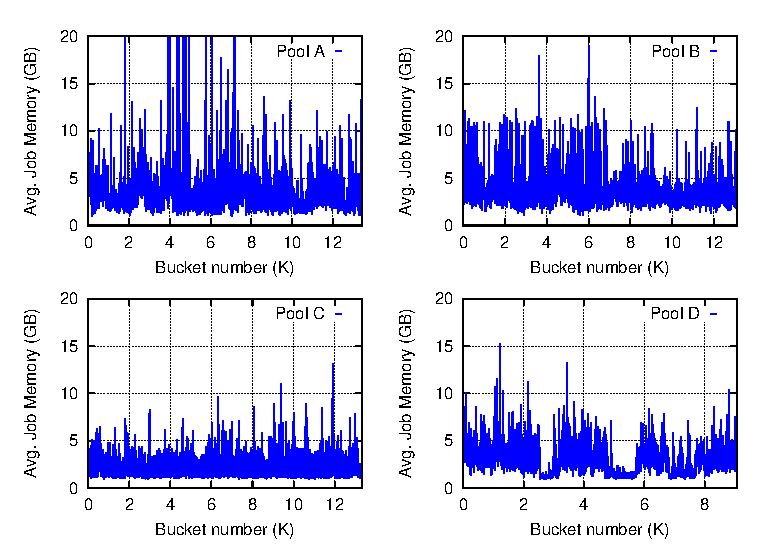
\includegraphics{figures/memory_burst.eps}
\caption{Bursts in jobs memory requirements: pools A and B are the
  most bursty; A in particular has bursts that exceed 20 GB on average.
  Pool C is somewhat steadier, while pool D exhibits periods of
  particularly low memory demands between the bursts.}
\label{fig:memory_burst_multiplot}
\end{figure}

Figures \ref{fig:cores_burst_multiplot} and
\ref{fig:memory_burst_multiplot} show the jobs' average cores and
memory requirements in each of the buckets, for each of the four pools,
respectively.
As can be seen, different pools exhibit different magnitudes of bursts
of jobs with high core or memory demands.
Pool A is the most bursty in both dimensions; it is the only pool that
had a bucket in which the average job core requirement is higher than
2, and multiple buckets in which the average memory requirement is
larger than 20 GB.

Pool B exhibits sparse bursts of jobs with high core demands, but
intense bursts of high memory requirements.
Pool C exhibits continuous moderate core demands, and also relatively
steady memory bursts.
Finally, pool D has virtually no bursts of jobs requiring more than
one core, but it does exhibit bursts of high memory demands, along
with periods of particularly low memory requirements.


\section{Comparing Heuristics}\label{sec:buckets}
%--------------------------------

To demonstrate the effectiveness of the different heuristics under different workloads 
we performed the following experiment.
We used the buckets described above, assigned all jobs in each bucket a submit
time of 0, and gave each heuristic an opportunity to try and match, in simulation, 
as many jobs as possible from each bucket on a small synthetic pool of
empty machines (total of 512 cores);
jobs that could not be matched were simply skipped.
For each bucket we then counted the number of jobs matched by each heuristic, 
and gave the winning heuristic(s) (the one(s) who matched the highest
number of jobs) a point.

%Given that each bucket contains tens of thousands of jobs, they
%cannot all be assigned to machines.

%We repeated the experiment four times: first on three homogeneous
%clusters in which all machines use the same number of cores and
%memory, and then on a heteserogeneous cluster containing a mixture of
%machines from the aforementioned clusters.

The results are shown in Figure \ref{fig:buckets}.
As can be seen, \wfc\ significantly outperforms all other heuristics 
(collecting the highest percentage of wins) in pool A. 
It is also the best heuristic in pools B, C, and D, 
but the differences there are smaller.
There is little difference among \bfm, \wfm, and \bfc, although
\wfm\ is consistently slightly better than the other two.
Notably, for pool D where there is virtually no core fragmentation 
as indicated in Figure \ref{fig:cores_burst_multiplot}
there seems to be little difference between the performance of the
different heuristics.

%This may indicate that it is best to first spread out the jobs across
%as many machines as possible.
%In fact, when all jobs are serial, \wfc\ is essentially the same as
%mapping jobs to machines in a round-robin manner.

\begin{figure}\centering                      
	\includegraphics[width=.9\textwidth]{figures/buckets-all-no-mf.eps}
\caption{\label{fig:buckets}Percentage of wins by each heuristic:
  \wfc\ significantly outperforms the other heuristics in pool A. The
  differences in pools B, C, and D are smaller.}
\end{figure}

An important observation is that though \wfc\ appears to be the preferred heuristic, 
it did \textit{not} win in all cases. 
This is shown by the gap between the \wfc\ bars 
and the 100\% mark, indicating that in 6--37\% of the experiments
other heuristics performed better. 
These gaps are the motivation for the \mif\ heuristic
proposed next. 


\chapter{\mif}
%=============
\label{sec:mixed-fit}

As demonstrated in the previous section, none of the one-dimensional
heuristics is capable of maximizing the number of matched jobs under
all workload scenarios.
In this section we propose a new heuristic, \mif, that takes into
account both cores and memory in an attempt to overcome the problem.


\section{Balanced Resource Usage}
%-----------------------------------

The basic idea behind \mif\ is to try and reach balanced resource
utilization across both cores and memory.
This is achieved by considering the \textit{configured} ratio of cores
to memory on each machine, and matching the job with the machine on
which the ratio of \textit{used} cores to memory, together with this
job, is closest to the configured ratio.

To see how this is done, envision a grid representing possible
resource combinations (as was done in Figures \ref{fig:wf_better} and
\ref{fig:bf_better}).
Each column represents a CPU core, and each row a block of memory (the
sizes of such blocks are not really important as long as they are used
consistently; they should correspond to the smallest unit being
allocated).
Assuming that cores and memory blocks are assigned exclusively to
jobs, an allocation may be portrayed as a sequence of shaded squares
on this grid, where each job is represented by a sequence of
memory-squares in a specific core-column.

The configured ratio is represented by the diagonal of this grid, and
the used ratio by the line connecting the top-right point of the grid
with the top-right point of the last job.
\mif\ defines a parameter, $\alpha$, that denotes the angle between
these two lines.
Note that the used ratio is calculated after allocating the job being
considered, so machines on which this job does not fit are excluded
from the discussion.
\mif\ then matches the job with the machine with the minimal $\alpha$
value.
In case of a tie, the first machine with the minimal value is used.

Two important notes. First, The grid is drawn such that memory and
cores are normalized to the same scale in each machine separately, thereby
creating a square.
This prevents the scale from affecting the angle.
Second, the angle is based on lines emanating from the top right corner.
It is also possible to have a similar definition based on the origin
(i.e.\ the bottom-left corner).
Choosing the top-right corner leads to higher sensitivity when the
machine is loaded, which facilitates better precision in balancing the
resources in such cases.

Let's see an example. 
Three machines are available, each with 4 cores and 32 GB of memory.
Machine A already has one job with 24 GB, Machine B has 2 jobs
with 8 GB each, and Machine C has one job with 2 cores and 4 GB memory
and another job with 1 core and 4 GB memory.
The next job that arrives requires one core and 8 GB of memory.
The various $\alpha$ values of all three machines including the newly
arrived job are demonstrated in Figure \ref{fig:fig3}.
The machine selected by \mif\ in this case is B where
$\alpha=0$.

\begin{figure}\centering
	\includegraphics[width=0.75\textwidth]{figures/fig3.eps}
\caption{Example of various $\alpha$ angles calculated by \mif. The
selected machine in this case is B where $\alpha=0$.}
\label{fig:fig3}
\end{figure}

To demonstrate why this may be expected to improve over the previous
heuristics we will use the same examples we used above.
Consider Figure \ref{fig:wf_better}, where \wof\ yielded the best
match.
After matching the first 16 GB job with machine A, \mif\ will 
match the second 16 GB job with machine B, as this will lead to a
smaller $\alpha$ value as can be seen in Figure \ref{fig:fig4}.
It will then match the remaining 4 GB jobs with both machines
until all cores get utilized.
As can be seen in Figure \ref{fig:mf_final} the end result is identical
to \wof.

\begin{figure}\centering
\subfigure[\label{fig:fig4}Options for placing the 2'nd job. The angle
  on machine B is smaller.]{
	\includegraphics[width=0.45\textwidth]{figures/fig4.eps}}
~~~~
\subfigure[\label{fig:mf_final}Final allocation by \mif.]{
\includegraphics[width=0.45\textwidth]{figures/fig1b.eps}}
\caption{\mif\ behavior for the example in Figure \ref{fig:wf_better}.
  The end result is identical to \wof.}
\end{figure}

%\begin{figure}\centering
%	\includegraphics[width=0.45\textwidth]{figures/fig1b.eps}
%\caption{Jobs allocated by \mif\ for Example 1.}
%\label{fig:mf_final}
%\end{figure}

Next, lets re-examine Figure \ref{fig:bf_better} where \bef\ yielded the
best results.
In this scenario \mif\ will match the first three 8 GB jobs with
machine A, and then the 32 GB job with machine B, replicating the
behavior of \bef.
Note that $\alpha$ would have been the same for the second 8 GB,
whether it would have been matched on machine A or B.
But as noted above, in such cases the \fif\ heuristics is used as a
tie breaker and hence the job is matched with machine A.
As can be seen in Figure \ref{fig:mf_final2} the end result is
identical to \bef.

\begin{figure}\centering
	\includegraphics[width=0.45\textwidth]{figures/fig2b.eps}
\caption{Jobs allocated by \mif\ for the Example in Figure
  \ref{fig:bf_better}.
  The result is identical to \bef.}
\label{fig:mf_final2}
\end{figure}


\section{\mif's Results}
%------------------------------

To check the performance of \mif\ we repeated the buckets 
experiment from Section \ref{sec:buckets}, 
but this time including \mif\ in the set of competing heuristics.
The results are shown in Figure \ref{fig:buckets-all}.
As can be seen, \mif\ wins by only a small margin in pool A, 
performs similarly to \wfc\ in pools B and D, and is slightly outperformed by \wfc\ 
in pool C.

\begin{figure}\centering
	\includegraphics[width=.9\textwidth]{figures/buckets-all.eps}
\caption{Percentage of wins by each heuristic: \mif\ wins by only a
  small margin in pool A, performs similarly to \wfc\ in pools B and
  D, and is slightly outperformed by \wfc\ in pool C.}
\label{fig:buckets-all}
\end{figure}

These results are counterintuitive, since in a two-dimensional
environment of cores and memory, where both resources are subject to
sudden deflation by bursts of jobs with high demands, a reasonable
strategy would be to try and balance the usage between the resources,
in order to secure a safety margin against bursts of any kind.
This strategy, however, which \mif\ employs, seems to yield some
improvement only under the most bursty situations (pool A).
This leads us to default to a meta-heuristic, \maj, which is described
next.

%To try and quantify the magnitude of this gap, we checked how many
%jobs were scheduled in buckets that \mif\ did not have the best schedule.
%In each such bucket, we measured the delta of jobs between the best
%algorithm in that particular bucket and \mif.
%Figure \ref{fig:mf-damage} shows the results.
%The results are that
%in those cases where \mif\ is not the best, \mif\ schedules 25--48
%jobs less than the best algorithm on average, which is around 0.25\%
%of the pool capacity.
%In other words, the difference was insignificant and \mif\ was very
%close to the best result.

%\begin{figure}\centering
%	\includegraphics[width=0.45\textwidth]{figures/mf-damage.eps}
%\caption{Number of jobs the best algorithm schedules more than \mif\, in the
%cases that \mif\ was not the best.}
%\label{fig:mf-damage}
%\end{figure}


